\documentclass[conference]{IEEEtran}
\IEEEoverridecommandlockouts

\usepackage{cite}
\usepackage{amsmath,amssymb,amsfonts}
\usepackage{algorithm}
\usepackage{algorithmic}
\usepackage{graphicx}
\usepackage{textcomp}
\usepackage{xcolor}
\usepackage{listings}
\usepackage{hyperref}
\usepackage{booktabs}
\usepackage{tabularx}
\usepackage{array}
\usepackage{url}
\usepackage{balance}
\usepackage{tikz}
\usetikzlibrary{shapes.geometric,shapes.misc,arrows.meta,positioning,fit,backgrounds,calc}

\lstset{
  basicstyle=\ttfamily\scriptsize,
  breaklines=true,
  frame=single,
  numbers=left,
  numberstyle=\tiny,
  tabsize=2,
  captionpos=b,
  showstringspaces=false
}

% ── TikZ flowchart styles ──────────────────────────────────────────────────
\tikzset{
  fc_start/.style={
    draw, rectangle, rounded corners=5pt, fill=gray!28, thick,
    minimum width=3.0cm, minimum height=0.55cm,
    text centered, font=\scriptsize
  },
  fc_proc/.style={
    draw, rectangle, fill=blue!12,
    minimum width=3.0cm, minimum height=0.55cm,
    text centered, font=\scriptsize
  },
  fc_warn/.style={
    draw, rectangle, fill=red!12, dashed,
    minimum width=3.0cm, minimum height=0.55cm,
    text centered, font=\scriptsize
  },
  fc_dec/.style={
    draw, diamond, fill=orange!22, aspect=2.6,
    text centered, font=\scriptsize, inner sep=1pt
  },
  fc_arr/.style={-Stealth, thick},
}

\def\BibTeX{{\rm B\kern-.05em{\sc i\kern-.025em b}\kern-.08em
    T\kern-.1667em\lower.7ex\hbox{E}\kern-.125emX}}

\begin{document}

\title{VISHWAAS: A Trust-First Distributed VPN Management System\\
with Explicit Approval Workflows, Centralised Control, and TPM-Backed Key Security}

\author{
  \IEEEauthorblockN{Anurag Krishnashankar}
  \IEEEauthorblockA{
    \textit{Software Engineering} \\
    \textit{VISHWAAS Project} \\
    vishwaas@local
  }
}

\maketitle

% ─────────────────────────────────────────────────────────────────────────────
\begin{abstract}
Modern enterprise network management demands secure, auditable, and centrally
controlled VPN provisioning. Existing solutions such as Tailscale, Nebula, and
raw WireGuard deployments either sacrifice explicit human oversight in favour of
automated mesh formation or rely on static configuration files that scale poorly
across distributed infrastructure. VISHWAAS (\textit{Sanskrit: ``trust''}) is a
production-ready, approval-first VPN orchestration platform built on WireGuard,
FastAPI, and React. It enforces the invariant that \emph{no node may join the
VPN, and no peer connection may become active, without explicit administrator
approval}. This paper presents the system architecture, the two-tier
controller\slash{}agent topology, the cryptographic key-management model
(including optional TPM~2.0 hardware binding), complete lifecycle state machines
governing join and connection flows, formal algorithm specifications for approval
procedures, the REST API surface, the hub-and-spoke routing model for gateway
nodes, and the comprehensive audit-logging subsystem. We evaluate the system
against five formal design goals, analyse the security threat model, and identify
future directions including multi-administrator RBAC, automated key rotation, and
high-availability controller clustering.
\end{abstract}

\begin{IEEEkeywords}
WireGuard, VPN orchestration, zero-trust networking, TPM~2.0, approval workflow,
distributed systems, FastAPI, network security, audit logging
\end{IEEEkeywords}


% =============================================================================
\section{Introduction}
% =============================================================================

Virtual Private Networks (VPNs) remain a foundational technology for securing
communication across untrusted networks. The emergence of
WireGuard~\cite{donenfeld2017wireguard} as a lean, modern VPN protocol has
renewed interest in deploying mesh and hub-and-spoke overlay networks without the
operational overhead of IPsec or OpenVPN. Yet the tooling surrounding
WireGuard---static \texttt{wg-quick} files, peer-exchange daemons, or fully
automated mesh controllers---consistently makes a trade-off: \emph{ease of
configuration at the cost of explicit approval and auditability}.

In regulated industries (healthcare, finance, government) and zero-trust security
postures~\cite{zerotrust}, this trade-off is unacceptable. Network administrators
must be able to answer: \textit{Who approved this node joining our VPN?  When was
this peer connection established?  Who was the authorising principal?}  Existing
tooling provides either no answers or requires bolting on external audit systems.

VISHWAAS addresses these requirements through a central controller that acts as a
gated authority: every state transition (a node joining, two peers connecting, a
connection being terminated) requires explicit human approval and produces an
immutable audit-log entry.  The system couples this strict approval model with a
lightweight per-node agent that exposes a minimal HTTP API, enabling the
controller to translate approvals directly into live WireGuard configuration
changes without manual SSH or configuration management tools.

The name \textit{VISHWAAS} (Sanskrit: \textit{trust, confidence}) reflects the
project's philosophical foundation: trust must be explicitly granted, never
assumed.

\subsection{Contributions}

\begin{enumerate}
  \item A formal description of an approval-first VPN orchestration architecture
        with clear separation between control-plane (controller) and
        data-plane-adjacent (agent) components.
  \item Complete lifecycle state machine specifications for node join and peer
        connection flows, including atomicity guarantees and rollback semantics,
        expressed as algorithm pseudocode.
  \item An analysis of three key-management strategies---agent-generated,
        controller-issued, and TPM~2.0 hardware-bound---and their security
        trade-offs.
  \item A hub-and-spoke routing model with automatic IP forwarding and subnet
        advertisement, enabling scalable gateway topologies within WireGuard's
        routing model.
  \item A thorough security threat model covering token security, transport
        security, JWT lifecycle management, and TPM-bound key storage.
\end{enumerate}

\subsection{Paper Organisation}

Section~\ref{sec:background} reviews WireGuard fundamentals and related systems.
Section~\ref{sec:architecture} describes the overall system architecture.
Section~\ref{sec:lifecycle} details state machines and approval algorithms.
Section~\ref{sec:keymanagement} covers key-management strategies.
Section~\ref{sec:topology} describes the network topology model.
Section~\ref{sec:api} catalogues the REST API surface.
Section~\ref{sec:security} presents the security threat model.
Section~\ref{sec:implementation} summarises the implementation.
Section~\ref{sec:evaluation} evaluates the system.
Section~\ref{sec:limitations} identifies limitations.
Section~\ref{sec:conclusion} concludes.


% =============================================================================
\section{Background and Related Work}
\label{sec:background}
% =============================================================================

\subsection{WireGuard Protocol}

WireGuard~\cite{donenfeld2017wireguard,wireguard-linux} is a modern VPN protocol
operating at Layer~3. It uses Curve25519 for ephemeral Diffie-Hellman key
agreement, ChaCha20-Poly1305 for authenticated symmetric encryption, BLAKE2s for
hashing, and SipHash for hash-table keys. Each peer is identified solely by a
256-bit Curve25519 public key; there are no certificates, no CAs, and no
negotiation phase. Routing is governed by \emph{allowed-ips} ACLs per peer: any
packet whose destination IP falls within a peer's \texttt{allowed-ips} set is
encrypted and forwarded to that peer's UDP endpoint.

WireGuard is intentionally low-level: it manages cryptographic tunnelling but
provides \emph{no} mechanism for key distribution, peer discovery, connection
approval, or lifecycle management. These responsibilities fall entirely on
operators or higher-level orchestration systems---the gap that VISHWAAS fills.

\subsection{Related Work}

\textbf{Tailscale}~\cite{tailscale} is a commercial WireGuard-based mesh VPN. It
automates peer discovery and key distribution via its coordination server, with
access governed by ACL policies. Tailscale prioritises user experience---nodes
join with a single authentication token. However, the approval granularity is
coarse (per-device, not per-connection), and the coordination server is
centralised in Tailscale's cloud, introducing a third-party trust dependency.
VISHWAAS is entirely self-hosted and enforces per-connection approval.

\textbf{Nebula}~\cite{nebula} is an open-source overlay network from Slack. It
uses lighthouse-based UDP hole-punching for peer discovery and certificate-based
identity. Like static WireGuard tools, Nebula distributes certificates at
deployment time and provides no runtime approval workflow.  VISHWAAS provides
dynamic runtime approval that Nebula lacks.

\textbf{WireGuard-over-Kubernetes} solutions (e.g., Kilo, Calico WireGuard)
automate WireGuard interface management via Kubernetes CRDs. These solutions are
tightly coupled to Kubernetes and assume implicit trust between cluster nodes.
VISHWAAS targets bare-metal and VM deployments without requiring a container
orchestration layer.

\textbf{Infrastructure-as-Code tools} (Ansible/Terraform WireGuard roles) provide
reproducible provisioning but are push-based: they execute at deployment time and
cannot respond to dynamic node join events without re-running playbooks. VISHWAAS
provides a continuously running control loop with real-time response.

VISHWAAS occupies a unique position: a self-hosted, approval-first, audit-complete
WireGuard orchestration system with a web UI, designed for dynamic node
populations in regulated or security-sensitive environments.


% =============================================================================
\section{System Architecture}
\label{sec:architecture}
% =============================================================================

VISHWAAS is a two-tier distributed system illustrated in
Figure~\ref{fig:architecture}. The \textbf{controller} constitutes the central
authority: a FastAPI~\cite{fastapi} backend paired with a React\slash{}Vite
single-page application. The \textbf{agent} is a lightweight FastAPI service
deployed on every VPN node. Communication is asymmetric: agents initiate join
requests to the controller; the controller initiates all subsequent configuration
commands to agents. The WireGuard data plane operates entirely peer-to-peer,
bypassing the controller after provisioning.

% ── Figure 1: Architecture (spans both columns) ───────────────────────────
\begin{figure*}[!t]
\centering
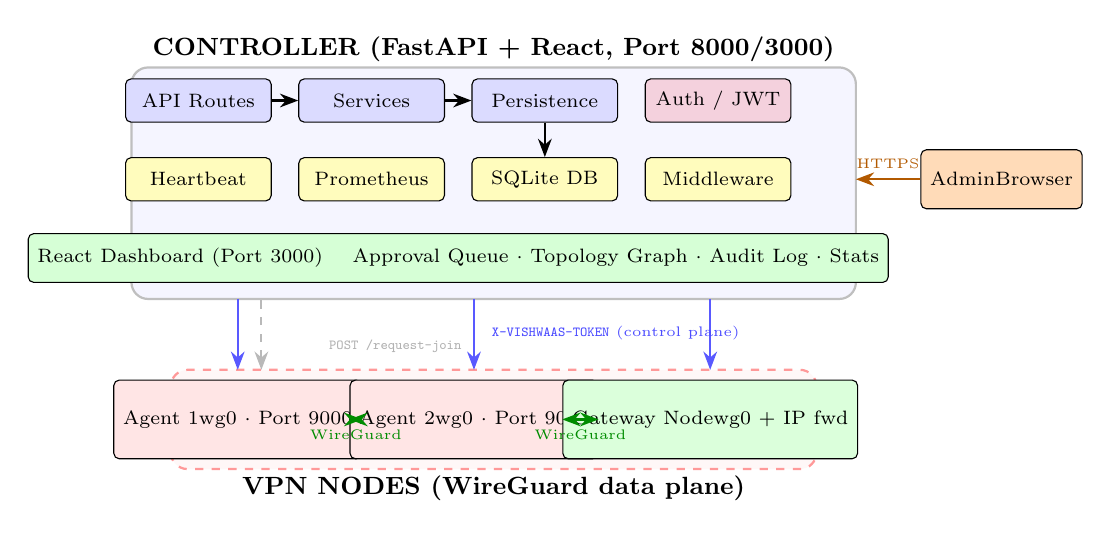
\begin{tikzpicture}[
  nd/.style={draw, rectangle, rounded corners=2pt, font=\scriptsize, text centered,
             minimum height=0.55cm},
  arr/.style={-Stealth, thick}
]

% ─── CONTROLLER bounding box (drawn first, lives behind nodes) ───
\filldraw[draw=gray!50, thick, rounded corners=6pt, fill=blue!4]
         (-0.85, 0.42) rectangle (8.35, -2.52);
\node[font=\small\bfseries] at (3.75, 0.65) {CONTROLLER (FastAPI + React, Port 8000/3000)};

% ─── Backend row ───
\node[nd, fill=blue!14, minimum width=1.85cm] (api)  at (0.0,  0.0) {API Routes};
\node[nd, fill=blue!14, minimum width=1.85cm] (svc)  at (2.2,  0.0) {Services};
\node[nd, fill=blue!14, minimum width=1.85cm] (pers) at (4.4,  0.0) {Persistence};
\node[nd, fill=purple!18, minimum width=1.85cm] (auth) at (6.6, 0.0) {Auth / JWT};

% ─── Infrastructure row ───
\node[nd, fill=yellow!26, minimum width=1.85cm] (hb)   at (0.0, -1.0) {Heartbeat};
\node[nd, fill=yellow!26, minimum width=1.85cm] (prom) at (2.2, -1.0) {Prometheus};
\node[nd, fill=yellow!26, minimum width=1.85cm] (db)   at (4.4, -1.0) {SQLite DB};
\node[nd, fill=yellow!26, minimum width=1.85cm] (corr) at (6.6, -1.0) {Middleware};

% ─── React frontend ───
\node[nd, fill=green!16, minimum width=9.0cm, minimum height=0.62cm] (fe)
     at (3.3, -2.0)
     {React Dashboard (Port 3000) \quad Approval Queue $\cdot$ Topology Graph $\cdot$ Audit Log $\cdot$ Stats};

% ─── Admin browser ───
\node[nd, fill=orange!28, minimum width=1.55cm, minimum height=0.75cm] (admin)
     at (10.2, -1.0) {Admin\\Browser};
% Arrow from admin to the right edge of the controller box
\draw[arr, orange!70!black] (admin.west) --
     node[above, font=\tiny] {HTTPS} (8.35, -1.0);

% ─── VPN NODES bounding box (behind agent nodes) ───
\filldraw[draw=red!40, thick, dashed, rounded corners=6pt, fill=red!3]
         (-0.35, -3.42) rectangle (7.85, -4.68);
\node[font=\small\bfseries] at (3.75, -4.92) {VPN NODES (WireGuard data plane)};

% ─── Agent nodes ───
\node[nd, fill=red!10, minimum width=2.4cm, minimum height=1.0cm] (ag1)
     at (0.5, -4.05) {Agent 1\\wg0 $\cdot$ Port 9000};
\node[nd, fill=red!10, minimum width=2.4cm, minimum height=1.0cm] (ag2)
     at (3.5, -4.05) {Agent 2\\wg0 $\cdot$ Port 9000};
\node[nd, fill=green!14, minimum width=2.4cm, minimum height=1.0cm] (agG)
     at (6.5, -4.05) {Gateway Node\\wg0 + IP fwd};

% ─── Internal controller flow arrows ───
\draw[arr] (api.east) -- (svc.west);
\draw[arr] (svc.east) -- (pers.west);
\draw[arr] (pers.south) -- (db.north);

% ─── Control-plane: controller → agents (blue solid) ───
\draw[arr, blue!65] (0.5, -2.52) -- (0.5, -3.42);
\draw[arr, blue!65] (3.5, -2.52) -- (3.5, -3.42);
\draw[arr, blue!65] (6.5, -2.52) -- (6.5, -3.42);
\node[font=\tiny, text=blue!70] at (5.3, -2.95)
     {\texttt{X-VISHWAAS-TOKEN} (control plane)};

% ─── Join-request: agents → controller (gray dashed) ───
\draw[{Stealth}-,  thick, gray!55, dashed] (0.8, -3.42) -- (0.8, -2.52);
\node[font=\tiny, text=gray!60] at (2.5, -3.12) {\texttt{POST /request-join}};

% ─── WireGuard data plane ───
\draw[{Stealth}-{Stealth}, thick, green!55!black]
     (ag1.east) -- (ag2.west) node[midway, below, font=\tiny] {WireGuard};
\draw[{Stealth}-{Stealth}, thick, green!55!black]
     (ag2.east) -- (agG.west) node[midway, below, font=\tiny] {WireGuard};

\end{tikzpicture}
\caption{VISHWAAS two-tier architecture. Blue solid arrows: controller-initiated peer-management
commands (authenticated via \texttt{X-VISHWAAS-TOKEN}). Dashed arrow: agent-initiated join
request (unauthenticated; secured by the explicit approval gate). Green arrows: WireGuard
encrypted data-plane tunnels established after approval, bypassing the controller entirely.
The controller manages all state; agents translate approved state into live WireGuard kernel calls.}
\label{fig:architecture}
\end{figure*}

\subsection{Controller Architecture}

The controller is structured into five functional layers:

\begin{itemize}
  \item \textbf{API Routes} (\texttt{app/api/routes/}): HTTP request handling and
        input validation via Pydantic schemas. Rate limiting is applied to all
        public endpoints.
  \item \textbf{Services} (\texttt{app/services/}): Stateless business logic for
        join approval, connection approval, agent communication, and audit
        logging.
  \item \textbf{Persistence} (\texttt{app/persistence/}):
        SQLAlchemy~\cite{sqlalchemy} ORM models and a SQLite database, providing a
        durable record of all nodes, requests, connections, and log events.
  \item \textbf{Domain} (\texttt{app/domain/enums.py}): Enumerated types encoding
        all valid states and event types, preventing illegal state transitions at
        the Python type system level.
  \item \textbf{Core} (\texttt{app/core/}): Application configuration (loaded from
        environment variables with the \texttt{VISHWAAS\_} prefix), JWT
        authentication utilities, heartbeat task, Prometheus metrics, and
        correlation middleware.
\end{itemize}

The \texttt{AgentClient} service encapsulates all HTTP calls from the controller
to individual agents. It uses a shared \texttt{httpx} connection pool with
exponential-backoff retry (up to 2 retries at 1\,s and 2\,s delays) and forwards
the \texttt{X-Request-ID} correlation header to all downstream agent calls.

\subsection{Agent Architecture}

The agent is intentionally minimal: it translates HTTP commands from the
controller into WireGuard kernel system calls. Its components are:

\begin{itemize}
  \item \textbf{Main} (\texttt{app/main.py}): FastAPI application entry point.
        Manages startup keypair generation, the background join-retry loop, and
        all HTTP endpoint handlers.
  \item \textbf{WireGuard} (\texttt{app/wireguard.py}): Wraps \texttt{wg} and
        \texttt{ip} CLI commands. Provides idempotent operations:
        \texttt{provision\_interface}, \texttt{add\_peer}, \texttt{remove\_peer},
        \texttt{bring\_down}.
  \item \textbf{State} (\texttt{app/state.py}): Thread-safe state machine with
        four states: \texttt{WAITING}, \texttt{APPROVED}, \texttt{ACTIVE},
        \texttt{ERROR}. State is persisted to \texttt{agent\_state.json} on disk
        so agent restarts do not lose state.
  \item \textbf{Security} (\texttt{app/security.py}): Validates the
        \texttt{X-VISHWAAS-TOKEN} header on all token-gated endpoints.
  \item \textbf{TPM} (\texttt{app/tpm.py}): Optional hardware-backed key storage
        via TPM~2.0 Non-Volatile memory indices.
  \item \textbf{Logger} (\texttt{app/logger.py}): Structured logging to both
        \texttt{stderr} and a rotating file, with optional JSON output.
\end{itemize}

\subsection{Database Schema}

The controller persists all state in a SQLite database with seven tables:

\begin{table}[ht]
\caption{Database Schema Summary}
\label{tab:schema}
\centering
\small
\begin{tabular}{ll}
\toprule
\textbf{Table} & \textbf{Key Columns} \\
\midrule
\texttt{nodes} & id, name, public\_key (unique), vpn\_ip (unique), \\
               & agent\_url, status, is\_gateway, last\_seen \\
\texttt{join\_requests} & id, node\_name, public\_key, agent\_url, status, \\
                        & requested\_at \\
\texttt{connection\_requests} & id, requester\_id, target\_id (FK nodes), status \\
\texttt{connections} & id, node\_a\_id, node\_b\_id (FK nodes), status \\
\texttt{notifications} & id, type, message, is\_read, created\_at \\
\texttt{logs} & id, event\_type, description, performed\_by, created\_at \\
\texttt{revoked\_tokens} & id, jti, expires\_at \\
\bottomrule
\end{tabular}
\end{table}

The \texttt{logs} table is append-only by architectural convention: no service
layer method updates or deletes log entries. The \texttt{revoked\_tokens} table
implements a JWT blacklist; expired entries are pruned at controller startup.


% =============================================================================
\section{Lifecycle State Machines}
\label{sec:lifecycle}
% =============================================================================

\subsection{Node Join Lifecycle}

Figure~\ref{fig:join_flow} presents the complete join lifecycle flowchart.  The
join process proceeds in three phases: \emph{registration}, \emph{approval}, and
\emph{provisioning}.

\textbf{Phase 1 — Registration.} At startup the agent generates a WireGuard
keypair idempotently (existing keys on disk are retained across restarts), detects
its local IP, and enters the background join loop. The loop issues
\texttt{POST /request-join} to the controller with the node name, public key, and
advertised agent URL. If the controller finds a duplicate public key (previously
approved node that restarted), it tears down all active connections on peer
agents, deletes the stale node record, and creates a fresh \texttt{PENDING}
request---requiring the administrator to re-approve. This prevents stale
WireGuard peer entries from persisting across agent restarts.

\textbf{Phase 2 — Approval.} The administrator reviews the pending request in the
dashboard, inspects the node name, public key fingerprint, and agent URL, and
clicks \emph{Approve}. Algorithm~\ref{alg:join_approval} specifies the atomic
approval procedure executed by \texttt{join\_service.approve\_join\_request()}.

\textbf{Phase 3 — Provisioning.} On receipt of \texttt{POST /set-vpn-address}, the
agent calls \texttt{wireguard.provision\_interface(vpn\_ip)}, which creates or
reconfigures the \texttt{wg0} interface, assigns the VPN IP, and brings the link
up. After successful provisioning, the agent transitions to \texttt{ACTIVE} state
and the join retry loop terminates.

% ── Algorithm 1: Join Approval ──
\begin{algorithm}[!t]
\caption{Join Approval Procedure}
\label{alg:join_approval}
\begin{algorithmic}[1]
\REQUIRE $r$: \texttt{JoinRequest} with $r.\textit{status} = \textsc{Pending}$
\STATE Verify $r.\textit{status} = \textsc{Pending}$; abort with 409 otherwise
\STATE $\textit{vpn\_ip} \leftarrow$ first unallocated address in $[10.10.10.2,\;10.10.10.254]$
\STATE \textbf{INSERT} \texttt{Node}($r.\textit{name}$, $r.\textit{pubkey}$,
       $\textit{vpn\_ip}$, \textsc{Approved})
\STATE \textbf{UPDATE} $r.\textit{status} \leftarrow \textsc{Approved}$
\STATE \textbf{APPEND} $\texttt{LOG}(\textsc{Join\_Approved},\;\textit{timestamp})$
\STATE \textbf{async}: \texttt{POST /set-vpn-address} to $r.\textit{agent\_url}$
\STATE \quad Retry $\leq 4$ times at 5\,s intervals on network failure
\STATE \quad On agent ACK: \textbf{UPDATE} $\textit{node.status} \leftarrow \textsc{Active}$
\STATE \quad On all retries exhausted: leave node in \textsc{Approved};
       admin may retry via \texttt{POST /nodes/\{id\}/push-vpn-address}
\end{algorithmic}
\end{algorithm}

% ── Figure 2: Join lifecycle flowchart ──────────────────────────────────────
\begin{figure}[!t]
\centering
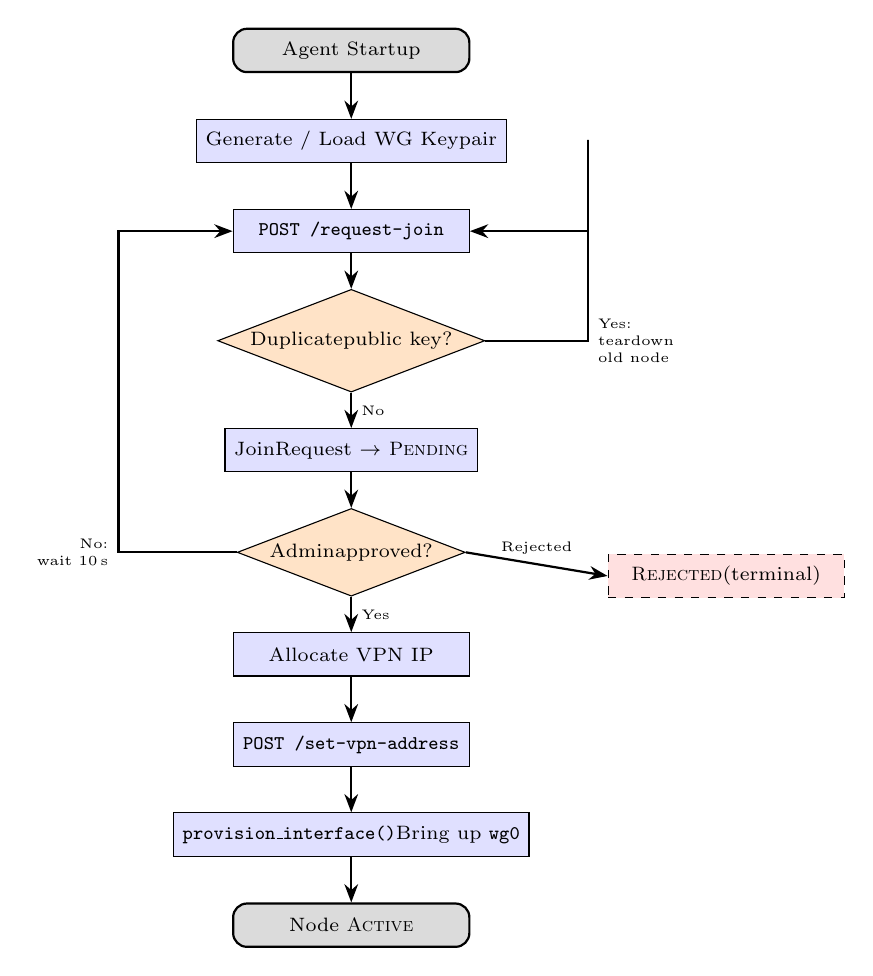
\begin{tikzpicture}[node distance=0.58cm]

\node[fc_start] (start) {Agent Startup};
\node[fc_proc,  below=of start]  (genkey)  {Generate / Load WG Keypair};
\node[fc_proc,  below=of genkey] (joinreq) {\texttt{POST /request-join}};
\node[fc_dec,   below=0.45cm of joinreq]   (dupkey)  {Duplicate\\public key?};
\node[fc_proc,  below=0.45cm of dupkey]    (pending) {JoinRequest $\rightarrow$ \textsc{Pending}};
\node[fc_dec,   below=0.45cm of pending]   (appd)    {Admin\\approved?};
\node[fc_proc,  below=0.45cm of appd]      (allocip) {Allocate VPN IP};
\node[fc_proc,  below=of allocip]          (pushvpn) {\texttt{POST /set-vpn-address}};
\node[fc_proc,  below=of pushvpn]          (provif)  {\texttt{provision\_interface()}\\Bring up \texttt{wg0}};
\node[fc_start, below=of provif]           (active)  {Node \textsc{Active}};

% Main flow arrows
\draw[fc_arr] (start)   -- (genkey);
\draw[fc_arr] (genkey)  -- (joinreq);
\draw[fc_arr] (joinreq) -- (dupkey);
\draw[fc_arr] (dupkey)  -- node[right, font=\tiny] {No} (pending);
\draw[fc_arr] (pending) -- (appd);
\draw[fc_arr] (appd)    -- node[right, font=\tiny] {Yes} (allocip);
\draw[fc_arr] (allocip) -- (pushvpn);
\draw[fc_arr] (pushvpn) -- (provif);
\draw[fc_arr] (provif)  -- (active);

% Duplicate key branch (right side loop back)
\draw[fc_arr] (dupkey.east) -- ++(1.3,0)
     node[right, font=\tiny, align=left] {Yes:\\teardown\\old node}
     -- ++(0, 2.55) |- (joinreq.east);

% Not yet approved (left side retry loop)
\draw[fc_arr] (appd.west) -- ++(-1.5,0)
     node[left, font=\tiny, align=right] {No:\\wait 10\,s}
     |- (joinreq.west);

% Rejection terminal
\node[fc_warn, right=1.8cm of appd, yshift=-0.3cm] (rej) {\textsc{Rejected}\\(terminal)};
\draw[fc_arr] (appd.east) -- node[above, font=\tiny] {Rejected} (rej.west);

\end{tikzpicture}
\caption{Node join lifecycle. The agent retries \texttt{POST /request-join} every 10\,s
until approved or rejected. A duplicate public key (agent restart) triggers automatic teardown
of the prior node before a fresh request is created, requiring administrator re-approval.}
\label{fig:join_flow}
\end{figure}

The full agent state machine is:
$\textsc{Waiting} \rightarrow \textsc{Approved}$ (on controller push)
$\rightarrow \textsc{Active}$ (after interface provisioning).
Rejection leads to a terminal \texttt{WAITING} state with no further retry.

\subsection{Connection Lifecycle}

Figure~\ref{fig:conn_flow} illustrates the connection lifecycle. Two nodes may
only be peered after explicit administrator approval.

\textbf{Request.} An administrator selects two nodes and submits
\texttt{POST /request-connection}.  The controller creates a
\texttt{ConnectionRequest} record (status \textsc{Pending}) and logs a
\texttt{CONNECTION\_REQUESTED} event. A second request for the same pair while
one is already \textsc{Pending} is idempotently rejected.

\textbf{Approval.} On administrator approval, Algorithm~\ref{alg:conn_approval}
specifies the atomic procedure executed by
\texttt{connection\_service.approve\_connection()}. The key invariant is
\emph{all-or-nothing}: if the second \texttt{add\_peer} call fails, the first is
rolled back immediately. No half-active connections are persisted.

\textbf{Termination.} An administrator terminates a connection via
\texttt{DELETE /connections/\{id\}}.  The controller calls
\texttt{DELETE /peer} on both agents to remove each other from the WireGuard peer
table, then marks the \texttt{Connection} as \textsc{Terminated}.  Critically,
the WireGuard interface (\texttt{wg0}) remains up on both nodes after termination:
the nodes stay on the VPN with their assigned IPs, simply no longer peered with
each other.

% ── Algorithm 2: Connection Approval ──
\begin{algorithm}[!t]
\caption{Connection Approval Procedure}
\label{alg:conn_approval}
\begin{algorithmic}[1]
\REQUIRE $cr$: \texttt{ConnectionRequest} with $cr.\textit{status} = \textsc{Pending}$
\REQUIRE Nodes $A = cr.\textit{requester}$, $B = cr.\textit{target}$; both \textsc{Active}
\STATE Compute $\textit{aips}_A, \textit{aips}_B$ based on gateway flags
       (see Section~\ref{sec:topology})
\STATE $r_A \leftarrow$ \texttt{POST /peer} to $A.\textit{agent\_url}$
       with $(B.\textit{pubkey},\; \textit{aips}_B,\; B.\textit{endpoint})$
\IF{$r_A.\textit{error}$}
  \STATE \textbf{RETURN} HTTP~502 (no state written)
\ENDIF
\STATE $r_B \leftarrow$ \texttt{POST /peer} to $B.\textit{agent\_url}$
       with $(A.\textit{pubkey},\; \textit{aips}_A,\; A.\textit{endpoint})$
\IF{$r_B.\textit{error}$}
  \STATE \textbf{ROLLBACK}: \texttt{DELETE /peer} from $A.\textit{agent\_url}$
         with $B.\textit{pubkey}$ \COMMENT{atomicity}
  \STATE \textbf{RETURN} HTTP~502 (no state written)
\ENDIF
\STATE \textbf{INSERT} \texttt{Connection}($A$, $B$, \textsc{Active})
\STATE \textbf{UPDATE} $cr.\textit{status} \leftarrow \textsc{Approved}$
\STATE \textbf{APPEND} $\texttt{LOG}(\textsc{Connection\_Approved},\;\textit{timestamp})$
\IF{$A.\textit{is\_gateway}$ \OR $B.\textit{is\_gateway}$}
  \STATE \texttt{POST /ip-forward/enable} on the gateway node
\ENDIF
\end{algorithmic}
\end{algorithm}

% ── Figure 3: Connection lifecycle flowchart ─────────────────────────────
\begin{figure}[!t]
\centering
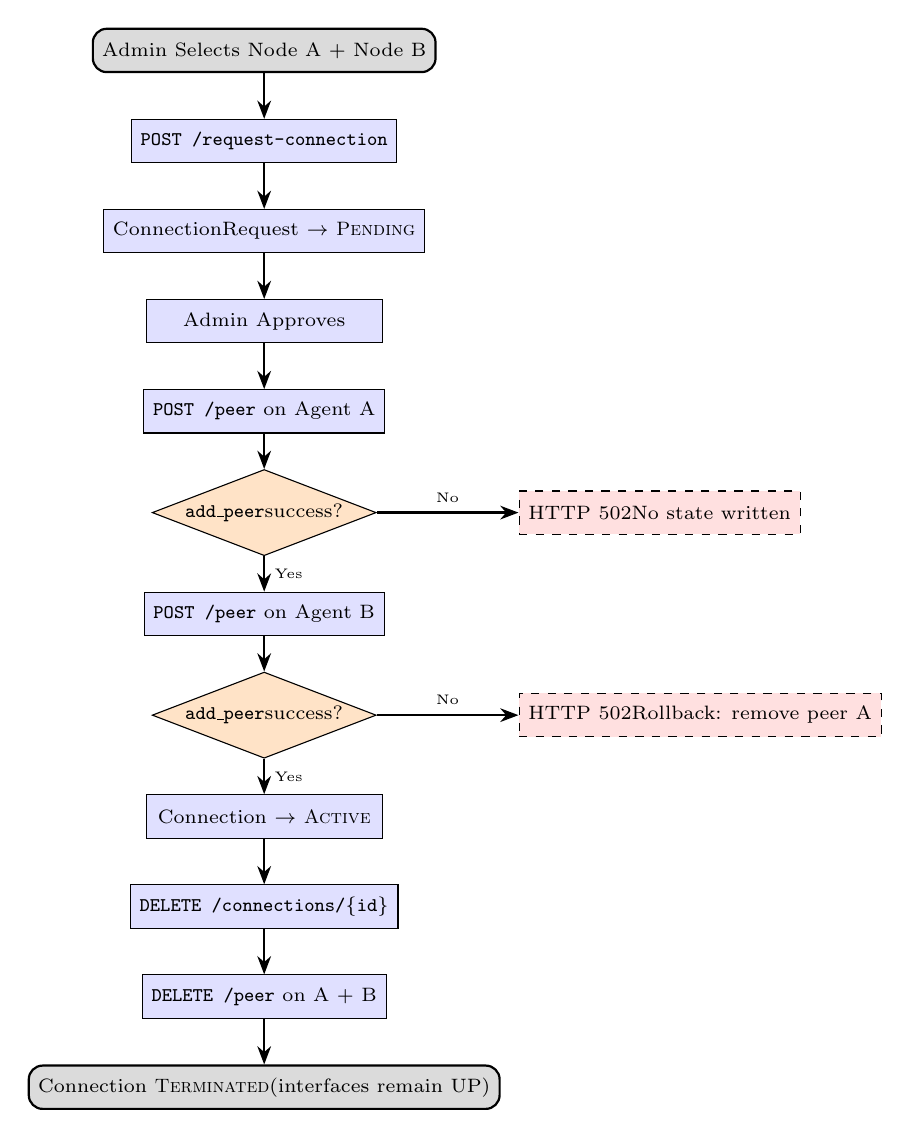
\begin{tikzpicture}[node distance=0.58cm]

\node[fc_start] (sel)    {Admin Selects Node A + Node B};
\node[fc_proc,  below=of sel]    (req)    {\texttt{POST /request-connection}};
\node[fc_proc,  below=of req]    (pend)   {ConnectionRequest $\rightarrow$ \textsc{Pending}};
\node[fc_proc,  below=of pend]   (appbtn) {Admin Approves};
\node[fc_proc,  below=of appbtn] (addA)   {\texttt{POST /peer} on Agent A};
\node[fc_dec,   below=0.45cm of addA]     (okA)    {\texttt{add\_peer}\\success?};
\node[fc_proc,  below=0.45cm of okA]      (addB)   {\texttt{POST /peer} on Agent B};
\node[fc_dec,   below=0.45cm of addB]     (okB)    {\texttt{add\_peer}\\success?};
\node[fc_proc,  below=0.45cm of okB]      (active) {Connection $\rightarrow$ \textsc{Active}};

% Termination branch
\node[fc_proc,  below=of active] (term1) {\texttt{DELETE /connections/\{id\}}};
\node[fc_proc,  below=of term1]  (term2) {\texttt{DELETE /peer} on A + B};
\node[fc_start, below=of term2]  (done)  {Connection \textsc{Terminated}\\(interfaces remain UP)};

% Error nodes
\node[fc_warn, right=1.8cm of okA] (errA) {HTTP 502\\No state written};
\node[fc_warn, right=1.8cm of okB] (errB) {HTTP 502\\Rollback: remove peer A};

% Main flow
\draw[fc_arr] (sel)    -- (req);
\draw[fc_arr] (req)    -- (pend);
\draw[fc_arr] (pend)   -- (appbtn);
\draw[fc_arr] (appbtn) -- (addA);
\draw[fc_arr] (addA)   -- (okA);
\draw[fc_arr] (okA)    -- node[right, font=\tiny] {Yes} (addB);
\draw[fc_arr] (addB)   -- (okB);
\draw[fc_arr] (okB)    -- node[right, font=\tiny] {Yes} (active);
\draw[fc_arr] (active) -- (term1);
\draw[fc_arr] (term1)  -- (term2);
\draw[fc_arr] (term2)  -- (done);

% Error branches
\draw[fc_arr] (okA.east) -- node[above, font=\tiny] {No} (errA.west);
\draw[fc_arr] (okB.east) -- node[above, font=\tiny] {No} (errB.west);

\end{tikzpicture}
\caption{Connection lifecycle with atomicity guarantees. If the second \texttt{add\_peer}
call fails, the first is immediately rolled back. No partial connection state is ever
persisted. On termination, both WireGuard interfaces remain up; only the peer table
entries are removed.}
\label{fig:conn_flow}
\end{figure}


% =============================================================================
\section{Key Management}
\label{sec:keymanagement}
% =============================================================================

VISHWAAS supports three distinct key-management strategies, selectable per agent.
Each offers a different trade-off between security, operational complexity, and
hardware requirements. Table~\ref{tab:keymanagement} summarises the comparison.

\subsection{Strategy 1: Agent-Generated Keys (Default)}

At startup the agent calls \texttt{wireguard.generate\_keypair()}, which shells
out to \texttt{wg genkey} and derives the public key via \texttt{wg pubkey}. Both
are written to \texttt{keys\_dir/\{privatekey,publickey\}} with permissions
\texttt{0600}/\texttt{0644}. The operation is idempotent: existing keys are
retained across restarts.

The private key \emph{never leaves the node}: the controller receives only the
public key in the join request body. This satisfies the principle of least
exposure.  The drawback is that a filesystem-level attacker with root access can
read the private key directly from disk.

\subsection{Strategy 2: Controller-Issued Keys}

Enabled by setting \texttt{"controller\_issues\_keys": true} in
\texttt{agent\_config.json}.  In this mode the agent submits the join request
with an empty public-key field; on approval, the controller generates a fresh
WireGuard keypair, stores the public key in the \texttt{Node} record, and
transmits the private key to the agent inside the \texttt{/set-vpn-address}
response body. This model centralises key generation but exposes the private key
in transit; it is only appropriate when the controller--agent channel is
TLS-encrypted.

\subsection{Strategy 3: TPM 2.0 Hardware-Bound Keys}

Enabled by setting \texttt{"use\_tpm\_wg\_key": true}. After generation (by
either Strategy~1 or Strategy~2), the agent calls
\texttt{tpm.write\_wg\_key\_to\_tpm(private\_key\_path, nv\_index)}, which:
\begin{enumerate}
  \item Runs \texttt{tpm2\_startup -c} to ensure a clean TPM~\cite{tpm2} context.
  \item Defines NV storage: \texttt{tpm2\_nvdefine -C o -s 45 -a
        ownerread|ownerwrite \{nv\_index\}}.
  \item Writes the 44-byte base64-encoded private key: \texttt{tpm2\_nvwrite -C o
        -i \{keyfile\} \{nv\_index\}}.
\end{enumerate}

Subsequently, every WireGuard call reads the key from TPM NV into a
\texttt{tempfile.NamedTemporaryFile} and immediately deletes it after use. This
prevents the private key from persisting on the filesystem. Even a full disk-image
exfiltration does not yield the WireGuard private key. If the TPM is unavailable,
the system falls back to disk-based access and logs a warning, preserving
availability at the cost of the hardware-binding property.

\begin{table}[ht]
\caption{Key Management Strategy Comparison}
\label{tab:keymanagement}
\centering
\begin{tabular}{lccc}
\toprule
\textbf{Property} & \textbf{Agent-Gen} & \textbf{Ctrl-Issued} & \textbf{TPM-Bound} \\
\midrule
Private key leaves node & No & Once & No \\
Key persists on disk    & Yes & Yes & No \\
Hardware binding        & No & No & Yes \\
Disk-dump resistant     & No & No & Yes \\
Requires TPM 2.0        & No & No & Yes \\
Agent complexity        & Medium & High & Low \\
Recommended use         & General & Dev/test & High-sec \\
\bottomrule
\end{tabular}
\end{table}


% =============================================================================
\section{Network Topology Model}
\label{sec:topology}
% =============================================================================

VISHWAAS supports three topology patterns governed by the \texttt{is\_gateway}
flag on node records.

\subsection{Peer-to-Peer Mesh}

When all nodes have $\texttt{is\_gateway} = \text{false}$, every approved
connection adds mutual \texttt{/32} peer entries on both sides.  The result is a
full or partial mesh.  Suitable for small networks (up to approximately 50 nodes
before the $O(n^2)$ peer-update overhead becomes significant) where low-latency
direct paths are required.

\subsection{Hub-and-Spoke (Gateway)}

A gateway node ($\texttt{is\_gateway} = \text{true}$) acts as a routing hub.
When a connection between spoke node~$S$ and gateway node~$G$ is approved:
\begin{itemize}
  \item \textbf{Spoke~$S$} receives \texttt{allowed-ips}~$= 10.10.10.0/24$ for
        peer~$G$, routing \emph{all} VPN traffic through~$G$.
  \item \textbf{Gateway~$G$} receives \texttt{allowed-ips}~$= S.\textit{vpn\_ip}/32$
        for peer~$S$.
  \item The controller enables kernel IP forwarding on~$G$ via
        \texttt{POST /ip-forward/enable} $\Rightarrow$ \texttt{sysctl -w
        net.ipv4.ip\_forward=1}.
\end{itemize}

This topology reduces the peer count from $O(n^2)$ (mesh) to $O(n)$, making it
suitable for large deployments. The hub handles all intra-VPN routing via the
kernel IP forwarding path.

\subsection{Hybrid Topology}

Multiple gateways can coexist with direct spoke-to-spoke meshes. The controller
computes \texttt{allowed-ips} correctly for each individual connection based on
the endpoint nodes' \texttt{is\_gateway} flags, enabling arbitrary hybrid
topologies. This computation is the core of \texttt{connection\_service}:

\begin{itemize}
  \item Both endpoints are spokes: $\texttt{allowed-ips} = \{\textit{peer.vpn\_ip}/32\}$ on each side.
  \item One endpoint is a gateway: spoke gets $\texttt{allowed-ips} = 10.10.10.0/24$; gateway gets $\texttt{allowed-ips} = \{\textit{spoke.vpn\_ip}/32\}$.
  \item Both endpoints are gateways: each gets $\texttt{allowed-ips} = 10.10.10.0/24$ for the other.
\end{itemize}

\subsection{Topology Visualisation}

The \texttt{GET /topology} endpoint returns a graph representation consumed by the
React dashboard, which renders it using \texttt{react-force-graph-2d}---a
physics-based force-directed layout that positions gateway nodes as visually
prominent hubs and spoke nodes as satellites:

\begin{lstlisting}[caption={Topology API response (abbreviated)}]
{
  "nodes": [
    { "id": 1, "name": "gw-1", "vpn_ip": "10.10.10.2",
      "status": "ACTIVE", "is_gateway": true },
    { "id": 2, "name": "node-a", "vpn_ip": "10.10.10.3",
      "status": "ACTIVE", "is_gateway": false }
  ],
  "edges": [
    { "id": 1, "source_id": 2, "target_id": 1,
      "status": "ACTIVE" }
  ]
}
\end{lstlisting}


% =============================================================================
\section{REST API Surface}
\label{sec:api}
% =============================================================================

\subsection{Controller API}

The controller exposes a comprehensive REST API on port~8000. All endpoints except
\texttt{POST /request-join} and \texttt{GET /health} require a valid JWT Bearer
token when authentication is enabled. Table~\ref{tab:controller-api} summarises
the primary endpoints.

\begin{table}[ht]
\caption{Controller REST API Surface (Selected Endpoints)}
\label{tab:controller-api}
\centering
\small
\begin{tabularx}{\columnwidth}{lX}
\toprule
\textbf{Method + Path} & \textbf{Description} \\
\midrule
POST /request-join & Agent submits join request (tokenless) \\
GET /join-requests & List requests, filterable by status \\
POST /join-requests/\{id\}/approve & Admin approves join \\
POST /join-requests/\{id\}/reject & Admin rejects join \\
\midrule
GET /nodes & List all nodes with pagination \\
GET /nodes/\{id\} & Node detail with WireGuard stats \\
PATCH /nodes/\{id\} & Update agent\_url or name \\
POST /nodes/\{id\}/push-vpn-address & Retry VPN address push \\
POST /nodes/\{id\}/set-gateway & Mark node as hub \\
DELETE /nodes/\{id\} & Remove node and teardown connections \\
\midrule
POST /request-connection & Request peer connection \\
POST /connection-requests/\{id\}/approve & Approve and activate peers \\
DELETE /connections/\{id\} & Terminate connection \\
\midrule
GET /stats & Dashboard summary counts \\
GET /stats/detailed & Per-node WireGuard bandwidth \\
GET /logs & Audit log (filterable by event type) \\
GET /topology & Graph nodes + edges \\
GET /notifications & Unread admin notifications \\
GET /health & Liveness probe \\
GET /ready & Readiness probe (DB connectivity check) \\
GET /metrics & Prometheus metrics endpoint \\
\midrule
POST /auth/login & Obtain JWT token \\
POST /auth/logout & Revoke JWT (add jti to blacklist) \\
GET /auth/me & Validate current session \\
\bottomrule
\end{tabularx}
\end{table}

\subsection{Agent API}

The agent exposes a minimal API on port~9000. All endpoints except
\texttt{GET /health} require the \texttt{X-VISHWAAS-TOKEN} header.

\begin{table}[ht]
\caption{Agent REST API Surface}
\label{tab:agent-api}
\centering
\small
\begin{tabularx}{\columnwidth}{lX}
\toprule
\textbf{Method + Path} & \textbf{Description} \\
\midrule
GET /health & Liveness check; returns agent state, wg interface stats \\
POST /set-vpn-address & Provision WireGuard interface with assigned IP \\
POST /peer & Add or update a WireGuard peer \\
DELETE /peer & Remove a WireGuard peer by public key \\
POST /wg/start & Bring WireGuard interface up \\
POST /wg/stop & Bring WireGuard interface down \\
GET /wg/status & Return current WireGuard interface stats \\
POST /ip-forward/enable & Enable kernel IPv4 forwarding \\
POST /remove-node & Full teardown (remove all peers, down interface) \\
\bottomrule
\end{tabularx}
\end{table}

\subsection{Uniform Response Envelope}

Both controller and agent return a consistent JSON envelope:

\begin{lstlisting}[caption={Unified response envelope}]
{ "success": true | false,
  "message": "Human-readable summary",
  "detail": "Optional debug info or null" }
\end{lstlisting}

HTTP status codes follow REST conventions: 200 for success, 400 for bad request,
401 for missing/invalid token, 404 for absent resource, 409 for conflict, 422
for Pydantic validation failures, 502 when the controller cannot reach an agent,
and 503 when configuration is missing.


% =============================================================================
\section{Security Analysis}
\label{sec:security}
% =============================================================================

\subsection{Authentication and Authorisation}

VISHWAAS employs three distinct authentication mechanisms:

\textbf{Agent-to-Controller (Join Request).} Join requests are intentionally
unauthenticated at the transport level---an agent presenting a join request is, by
definition, an unknown entity. Security is provided by the approval gate: the
administrator must inspect and explicitly approve the request before the node
receives any VPN configuration. The public key in the join request serves as a
cryptographic identity anchor; an adversary submitting a fraudulent request with a
different key will receive a different VPN IP and cannot impersonate an approved
node.

\textbf{Controller-to-Agent (Peer Management).} All controller calls to agent
endpoints carry an \texttt{X-VISHWAAS-TOKEN} header validated against the agent's
configured \texttt{master\_token}. A mismatch returns HTTP~401 and logs a
``suspicious access'' warning. This shared-secret model is simple and effective for
internal networks but does not provide per-message authentication or replay
protection.

\textbf{Dashboard (Administrator UI).} Authentication is controlled by the
\texttt{VISHWAAS\_ADMIN\_PASSWORD\_HASH} environment variable. When set, the
frontend obtains a JWT (HS256, configurable expiry defaulting to 480 minutes) via
\texttt{POST /auth/login}. The JWT carries a \texttt{jti} claim; logout adds the
\texttt{jti} to the \texttt{revoked\_tokens} table, blacklisting the token for its
remaining validity period. Expired blacklist entries are pruned at controller
startup.

\subsection{Transport Security}
\label{sec:transport}

VISHWAAS delegates transport security to the deployment environment. The
recommended production deployment places an nginx reverse proxy with TLS in front
of the controller API and serves agent URLs over HTTPS. Without TLS, the
\texttt{X-VISHWAAS-TOKEN}, JWT tokens, and (in controller-issued-key mode)
WireGuard private keys are transmitted in plaintext.

\subsection{Heartbeat and Liveness}

A background heartbeat task runs every 60 seconds, pinging all
\textsc{Active}/\textsc{Approved} nodes. After 90 seconds of silence, a node is
marked \textsc{Offline}; after 5 minutes, it is auto-deleted along with its
connections from the database. The heartbeat also checks agents with
\textsc{Pending} join requests and marks requests \textsc{Rejected} after 120
seconds of agent unreachability, preventing clutter in the approval queue. A
startup sweep runs one immediate pass at controller boot, marking unreachable nodes
\textsc{Offline} without waiting for the 90-second threshold.

\subsection{Threat Model}

Table~\ref{tab:threats} enumerates the primary threats, their risk levels under a
default HTTP deployment, and the available mitigations.

\begin{table}[ht]
\caption{Threat Model Summary}
\label{tab:threats}
\centering
\small
\begin{tabularx}{\columnwidth}{lllX}
\toprule
\textbf{Threat} & \textbf{Risk} & \textbf{Mit.} & \textbf{Mitigation} \\
\midrule
Rogue agent join         & Med  & Partial & Admin approval gate \\
MITM controller--agent   & High & No (HTTP) & Use HTTPS/TLS \\
Stolen agent token       & High & No      & Rotate token, use HTTPS \\
Private key exfiltration & Med  & Partial & TPM binding \\
JWT theft (localStorage) & Med  & Partial & HTTPS, short expiry, \texttt{jti} blacklist \\
SQL injection            & Low  & Yes     & SQLAlchemy ORM \\
XSS in dashboard         & Med  & Partial & React auto-escaping \\
Replay on agent API      & Med  & No      & Add nonce/timestamp \\
VPN IP pool exhaustion   & Low  & Yes     & Sequential allocation check \\
Rogue admin action       & Low  & Partial & Immutable audit log \\
\bottomrule
\end{tabularx}
\end{table}

\subsection{Audit and Non-Repudiation}

The \texttt{logs} table records every significant state transition with its
\texttt{event\_type}, human-readable \texttt{description}, optional
\texttt{performed\_by} principal, and a millisecond-precision \texttt{created\_at}
timestamp. Defined event types include: \texttt{JOIN\_REQUESTED},
\texttt{JOIN\_APPROVED}, \texttt{JOIN\_REJECTED}, \texttt{CONNECTION\_REQUESTED},
\texttt{CONNECTION\_APPROVED}, \texttt{CONNECTION\_REJECTED},
\texttt{CONNECTION\_TERMINATED}, \texttt{NODE\_REMOVED}, and
\texttt{NODE\_OFFLINE}. No service-layer code updates or deletes log entries,
providing a best-effort immutable audit trail. For cryptographic non-repudiation,
an external append-only log store (e.g., a Merkle-tree-based audit log) would be
required; this is identified as future work.


% =============================================================================
\section{Implementation}
\label{sec:implementation}
% =============================================================================

\subsection{Technology Stack}

\textbf{Controller Backend:} Python 3.10+, FastAPI~\cite{fastapi} 0.115+,
uvicorn 0.32+ (ASGI server), SQLAlchemy~\cite{sqlalchemy} 2.0+ ORM with SQLite
backend (configurable to PostgreSQL via \texttt{VISHWAAS\_DATABASE\_URL}),
Pydantic 2.0+ for request/response validation, python-jose + cryptography for JWT
(HS256), passlib + bcrypt for password hashing, httpx 0.27+ for async HTTP calls
to agents, prometheus-client for metrics exposure, Alembic for database
migrations.

\textbf{Agent:} Python 3.10+, FastAPI 0.109+, uvicorn 0.27+, \texttt{subprocess}
for \texttt{wg} and \texttt{ip} CLI invocations, \texttt{tpm2-tools} (optional)
for TPM NV operations, \texttt{tempfile} for secure ephemeral key handling.

\textbf{Frontend:} React~\cite{react} 18.3+, React Router 6.28+, Vite 5.4+
(build toolchain), \texttt{react-force-graph-2d} 1.29+ for topology
visualisation, Recharts 3.7+ for bandwidth charts, lucide-react 0.474+ for
iconography, React Context API for global state management.

\subsection{Deployment}

The recommended production deployment installs the agent as a systemd service at
\texttt{/opt/vishwaas-agent} via \texttt{install.sh}, enabling automatic start on
boot and restart on failure. The controller runs behind an nginx reverse proxy
configured for HTTPS, rate limiting, and restriction of the \texttt{/metrics}
endpoint to the VPN subnet. Database schema is managed by Alembic migrations;
existing deployments run \texttt{alembic stamp head} once to baseline before
upgrading.

\subsection{Codebase Metrics}

\begin{table}[ht]
\caption{Codebase Size Summary}
\label{tab:codebase}
\centering
\begin{tabular}{lrr}
\toprule
\textbf{Component} & \textbf{Files} & \textbf{Approx.\ LOC} \\
\midrule
Controller backend & 20 & $\sim$2{,}800 \\
Agent              &  8 & $\sim$1{,}200 \\
Frontend (JSX/JS)  & 16 & $\sim$1{,}500 \\
Scripts \& config  & 10 & $\sim$300 \\
\midrule
\textbf{Total (excl.\ vendored)} & \textbf{54} & \textbf{$\sim$5{,}800} \\
\bottomrule
\end{tabular}
\end{table}


% =============================================================================
\section{Evaluation}
\label{sec:evaluation}
% =============================================================================

We evaluate VISHWAAS against five design goals articulated at project inception.

\textbf{G1 — Explicit Approval.} Every node join and every peer connection requires
a positive administrator action. The state machines and database constraints ensure
no node can transition to \textsc{Active} without a recorded approval event.
Algorithm~\ref{alg:join_approval} and Algorithm~\ref{alg:conn_approval} specify
these guarantees formally. \textit{Met.}

\textbf{G2 — Immutable Audit Log.} All state transitions produce append-only log
entries with event type, principal, and timestamp. The absence of
update/delete operations on the \texttt{logs} table (enforced by convention across
all service modules) provides a complete record. \textit{Mostly met}; cryptographic
tamper-evidence requires an external append-only store.

\textbf{G3 — Zero-Touch Provisioning After Approval.} Once approved, the
controller automatically provisions the WireGuard interface on the agent without
any manual SSH or configuration file editing. Background retry logic handles
transient agent unavailability; administrators may trigger manual retries via the
dashboard. \textit{Met.}

\textbf{G4 — Key Security Commensurate with Hardware.} Three escalating strategies
are available: disk-based, controller-issued, and TPM-bound. TPM binding prevents
private-key exfiltration even under full disk compromise. \textit{Met.}

\textbf{G5 — Scalable Topology.} Hub-and-spoke topology with per-connection routing
policies reduces the peer-count complexity from $O(n^2)$ to $O(n)$ for
gateway-mediated networks. The topology API and force-graph visualisation enable
administrators to manage hundreds of nodes. \textit{Met for gateway topologies;
mesh topology has inherent $O(n^2)$ scaling.}


% =============================================================================
\section{Limitations and Future Work}
\label{sec:limitations}
% =============================================================================

\subsection{Current Limitations}

\begin{enumerate}
  \item \textbf{Single Administrator.} The authentication model supports a single
        \texttt{admin} account. Multi-user RBAC (e.g., read-only observers,
        scoped approvers) is absent.
  \item \textbf{No Key Rotation.} WireGuard keypairs are static for the lifetime
        of a node registration. Rotation requires deleting the node and
        re-joining, causing a brief VPN outage.
  \item \textbf{SQLite Single-Point-of-Failure.} SQLite does not support
        concurrent writes or replication. A controller failure takes down the
        management plane; the VPN data plane (WireGuard itself) continues
        operating unaffected.
  \item \textbf{IPv4 Only.} VPN addressing and routing are hardcoded to IPv4.
        IPv6 dual-stack is not supported.
  \item \textbf{No Mutual TLS.} Agent authentication relies on a shared token.
        A compromised token grants full control over all agents.
  \item \textbf{No Replay Protection on Agent API.} The
        \texttt{X-VISHWAAS-TOKEN} header provides authentication but not message
        freshness. A captured valid request could be replayed.
  \item \textbf{CORS Wildcard.} The controller sets
        \texttt{allow\_origins=["*"]} by default. This must be restricted for
        internet-facing controllers via \texttt{VISHWAAS\_ALLOWED\_ORIGINS}.
\end{enumerate}

\subsection{Future Work}

\begin{enumerate}
  \item \textbf{Multi-Admin RBAC.} Introduce roles (\textit{viewer},
        \textit{approver}, \textit{admin}) with fine-grained permissions.
        OAuth~2.0 / LDAP integration for enterprise identity providers.
  \item \textbf{Automated Key Rotation.} Zero-downtime rotation: generate a new
        keypair, propagate the new public key to all existing peers via the
        controller, activate the new interface, deactivate the old, and update
        the database atomically.
  \item \textbf{High-Availability Controller.} Migrate persistence to
        PostgreSQL, add a health-check endpoint, and deploy behind a load
        balancer with active/passive failover.
  \item \textbf{Prometheus Metrics Exporter.} Expose per-node bandwidth, active
        connections, pending approvals, and join-request queue depth in
        OpenMetrics format (partially implemented via \texttt{prometheus-client}).
  \item \textbf{Webhook Notifications.} Push approval events and node-status
        changes to configurable webhook URLs (Slack, Teams, PagerDuty) to
        integrate into NOC workflows.
  \item \textbf{Replay Protection.} Add a timestamp and nonce to
        controller$\rightarrow$agent requests with a short validity window to
        prevent replay attacks.
  \item \textbf{IPv6 Dual-Stack.} Extend the VPN addressing scheme to support
        IPv6 prefixes and dual-stack nodes.
  \item \textbf{Cryptographic Audit Log.} Integrate a Merkle-tree-based
        append-only log (e.g., Trillian) to provide cryptographic tamper
        evidence for the audit trail.
\end{enumerate}


% =============================================================================
\section{Conclusion}
\label{sec:conclusion}
% =============================================================================

VISHWAAS demonstrates that an approval-first VPN management system can be
practical, operationally useful, and architecturally clean without sacrificing the
security properties demanded by regulated environments. By treating every state
transition as a first-class event requiring explicit human authorisation, VISHWAAS
provides the auditability that automated mesh VPN systems inherently lack.

The two-tier controller/agent architecture cleanly separates the management concern
(who may join, who may connect to whom) from the configuration concern (how to
translate those decisions into WireGuard system calls). This separation enables the
agent to remain minimal and auditable---approximately 1\,200 lines of Python that
do exactly one thing---while the controller accumulates organisational knowledge
and approval history. The formal algorithm specifications in
Algorithms~\ref{alg:join_approval} and~\ref{alg:conn_approval} make the atomicity
guarantees explicit and verifiable.

The three-strategy key management model, culminating in TPM-bound hardware keys,
gives operators a path from simple development deployments to high-assurance
production deployments on the same codebase. The hub-and-spoke topology model
provides the routing scalability needed for real enterprise deployments without
sacrificing the approval-per-connection invariant.

VISHWAAS is a mature foundation for organisations wishing to deploy WireGuard-based
VPNs under strict operational discipline. Its primary gaps---single-admin, no key
rotation, SQLite persistence---are well-understood engineering problems with clear
solutions identified in the future-work roadmap. The core approval-workflow and
audit-logging infrastructure, the system's most distinctive contribution, is
complete and production-ready.

% =============================================================================
\section*{Acknowledgements}
% =============================================================================

The author thanks the WireGuard project~\cite{donenfeld2017wireguard} for
providing a principled and auditable VPN primitive on which VISHWAAS is built, and
the FastAPI project~\cite{fastapi} for enabling rapid development of
well-validated Python HTTP services.

\balance

% =============================================================================
\begin{thebibliography}{00}

\bibitem{donenfeld2017wireguard}
J.~A. Donenfeld, ``WireGuard: Next Generation Kernel Network Tunnel,''
in \textit{Proc. Network and Distributed System Security Symposium (NDSS)},
San Diego, CA, USA, Feb.\ 2017.

\bibitem{tailscale}
Tailscale Inc., ``How Tailscale Works,''
\textit{Tailscale Engineering Blog}, 2020.
[Online]. Available: \url{https://tailscale.com/blog/how-tailscale-works}

\bibitem{nebula}
Slack Technologies, ``Nebula: A Scalable Overlay Networking Tool,''
GitHub, 2019. [Online]. Available: \url{https://github.com/slackhq/nebula}

\bibitem{fastapi}
S.~Ramirez, ``FastAPI: Modern, Fast Web Framework for Building APIs with Python,''
GitHub, 2019. [Online]. Available: \url{https://fastapi.tiangolo.com}

\bibitem{tpm2}
Trusted Computing Group, ``TPM 2.0 Library Specification, Part 1: Architecture,''
TCG Specification, Revision 1.59, 2019.
[Online]. Available: \url{https://trustedcomputinggroup.org/resource/tpm-library-specification/}

\bibitem{wireguard-linux}
J.~A. Donenfeld, ``WireGuard: Fast, Modern, Secure VPN Tunnel,''
\textit{Linux Journal}, vol.~2018, no.~287, pp.~1--11, 2018.

\bibitem{zerotrust}
J.~Kindervag, ``Build Security Into Your Network's DNA: The Zero Trust Network Architecture,''
Forrester Research, Technical Report, 2010.

\bibitem{sqlalchemy}
M.~Bayer, ``SQLAlchemy: The Database Toolkit for Python,''
GitHub, 2006. [Online]. Available: \url{https://www.sqlalchemy.org}

\bibitem{react}
Meta Platforms Inc., ``React: A JavaScript Library for Building User Interfaces,''
GitHub, 2013. [Online]. Available: \url{https://react.dev}

\bibitem{kilo}
S.~P. Smith, ``Kilo: A Multi-Cloud Network Overlay Built on WireGuard and BGP,''
KubeCon Europe, 2019.

\end{thebibliography}

\end{document}
